\chapter{Chapter 3: System Design and Methodology}

\section{Arena Setup and Coordinate System}

The experimental arena is a domestic garage measuring 6230~mm in the X direction (depth from the camera-north wall to the south wall), 3050~mm in the Y direction (width), and 2950~mm in the Z direction (height). The world-frame origin is taken at the North-East floor corner of the arena, with the \textbf{X-axis} pointing from the North wall toward the South wall (increasing toward the launcher end), the \textbf{Y-axis} pointing from the East wall toward the West wall, and the \textbf{Z-axis} pointing vertically upward. All coordinates in this thesis are in millimetres. The athlete operates in the central region of the arena, approximately between $X=2500$~mm and $X=5000$~mm.

\begin{table}[htbp]
\caption{Camera positions in world-frame coordinates (mm)}
\label{tab:3_1}
\begin{tabular}{|c|c|c|c|p{3.5cm}|}
\hline
\textbf{Camera} & \textbf{X (mm)} & \textbf{Y (mm)} & \textbf{Z (mm)} & \textbf{Description} \\
\hline
CamNorth & 50 & 1100 & 2260 & North wall, central height \\
\hline
CamEast & 1620 & 50 & 2120 & East wall, near North end \\
\hline
CamWest & 1600 & 2970 & 2170 & West wall, near North end \\
\hline
CamSouth & 6180 & 1530 & 2270 & South wall, central \\
\hline
\end{tabular}
\end{table}

The four cameras are mounted at ceiling height near the perimeter walls to provide overlapping fields of view across the central arena volume where the athlete operates. The placement was chosen to maximise the number of cameras simultaneously observing any operating-area target, with a nominal design objective of three or more cameras with clear visibility of the athlete at any operational position.

Twenty-four AprilTag fiducial markers (IDs 0--23, 21.5~cm $\times$ 21.5~cm) are affixed to the arena walls at pre-measured world-frame positions. Their coordinates are stored in the extrinsics calibration file and are used during the extrinsic-calibration process described in Section~3.5.

\section{Hardware Architecture}

\subsection{Cameras}

The four cameras are Hikvision DS-E12 USB webcams operating at 1280~$\times$~720 at a target capture rate of 15~FPS. They are consumer-grade fixed-focus cameras with no hardware synchronisation signal; software synchronisation by flashlight marker frames is used instead (Section~3.6). Each camera costs approximately USD~30.

\subsection{BLM Mechanical Architecture}

The Ball Launching Machine is a 2-DOF gimbal-mounted projectile launcher with a counter-rotating flywheel pair as the propulsion mechanism and a stepper-driven pusher as the feeder.

\textbf{Chassis.} The frame is built from 30~$\times$~30~mm aluminium 6061 extrusion with bolted corner brackets. Aluminium was preferred over the wood prototype of the precursor laboratory platform because the recoil from the pusher stroke and the reaction torque of the flywheels at $>$~800~RPM excite a vibration spectrum that wood damps poorly, and because the extrusion system makes the chassis re-configurable during iterative bring-up.

\textbf{Two-degree-of-freedom gimbal.} Two NEMA-23 stepper motors actuate the pitch and yaw axes through 1:50 worm-gear reducers. The worm-gear topology is chosen because it is \textbf{self-locking}: external torque at the output cannot back-drive the input. This means that on power loss the gimbal holds its aim without electrical holding current, which is a load-bearing safety property: a ball in the feeder cannot drop the barrel to an unsafe angle when the rail is interrupted. Approximately 2$^\circ$ of mechanical backlash is present on the horizontal reducer; this is compensated in software in the supervisor by tracking the last-commanded direction per axis and applying a one-sided dead-band on direction reversal. The working ranges are pitch $\in [0^\circ, +30^\circ]$ and yaw $\in [-30^\circ, +30^\circ]$, enforced both in the Python supervisor (primary) and the firmware command parser (secondary). Empirically, \texttt{set} commands with magnitudes beyond $\pm 30^\circ$ trigger an ESP32 reboot; the supervisor-side clamp therefore also functions as a crash-prevention interlock.

\textbf{Flywheel pair.} Two counter-rotating brushless DC (BLDC) wheels squeeze the ball at the pinch point. Differential left-right RPM imparts spin, generating a Magnus-effect lateral force in flight. Controlled fire has been qualified at 500--800~RPM (Section~5.9 and Appendix~A); the empirical RPM-to-exit-velocity calibration above 800~RPM is identified as future work in Section~6.4.

\textbf{Pusher and feeder.} The pusher is driven by a Texas Instruments DRV8825 stepper driver \cite{ref42_drv8825}, which supplies up to 2.5~A per phase, supports up to 1/32 micro-stepping, and includes integrated thermal shutdown and a current-limit potentiometer. The DRV8825's \texttt{nENABLE} pin is held HIGH (driver disabled, coil de-energised) while the firmware finite-state machine is in IDLE, and only pulled LOW (driver enabled) during RETRACTING, DISPENSING, or SHOOTING. This thermal-management discipline keeps the pusher coil cold between shots, extending motor life and reducing chassis thermal load. Three mechanical limit switches sense the pusher state: \textit{front} (ball released), \textit{back} (pusher retracted home), and \textit{ball} (magazine has a ball in position). All three are wired with the ESP32's internal \texttt{INPUT\_PULLUP} and triggered on LOW (closed-contact-to-GND). This polarity is chosen over PULLDOWN-HIGH because a broken wire then fails to the ``unpressed'' (HIGH) state, which is the safe default for motion interlocks. A hobby servo on the dispense flap, addressed by the \texttt{js} command, is angle-tunable at run-time via \texttt{jsset} without reflashing.

\textbf{Power architecture.} The ESP32 logic rail is powered from USB (5~V, supplied by the host PC). The motor rail is a fused 24~V supply (50~A fuse sized per IEC~60204-1 \cite{ref45_iec60204}) feeding the BLDC ESCs and the stepper drivers through separate breakers. Logic ground (USB GND) is tied to motor ground at a single star point on the base plate to prevent ground loops. A normally-closed mushroom-switch E-STOP latches the motor supply off in $<$~100~ms; the ESP32 remains powered via USB so that the supervisor can read \texttt{info} and log the event after the latch. Release requires both a manual \texttt{clear} command at the supervisor and a physical reset of the E-STOP, enforcing the ISO~13849-1 \cite{ref44_iso13849} two-action release principle.

\subsection{ESP32 Microcontroller}

The launcher state machine and motor control run on a single ESP32 microcontroller \cite{ref43_esp32} that receives serial commands from the host PC and translates them into stepper pulses, ESC PWM, and servo angles. The ESP32 was chosen over an Arduino UNO because (i) its dual cores allow the command parser and telemetry to run on one core while interrupt service routines (stepper step generation, limit-switch debouncing) run on the other; (ii) the 240~MHz clock is sufficient for 1/32 micro-step pulse cadence with head-room; (iii) the hardware UART is configurable above 1~Mbaud, enabling the 921~600~baud link selected in Section~3.11; and (iv) the on-chip BLE radio remains available as a backup channel without changes to the hardware design.

The command set received over the serial link is summarised in Table~\ref{tab:3_2}; the underlying firmware finite-state machine is described in Section~3.10.

\begin{table}[htbp]
\caption{BLM low-level serial command set}
\label{tab:3_2}
\centering
\begin{tabularx}{\textwidth}{|l|l|X|}
\hline
\textbf{Command} & \textbf{Syntax} & \textbf{Effect} \\
\hline
set & \texttt{set V H WL WR} & Set vertical (pitch) angle V (degrees), horizontal (yaw) angle H (degrees), left-wheel RPM WL, and right-wheel RPM WR \\
\hline
shoot & \texttt{shoot} & Trigger one ball-ejection cycle (firmware-gated by RPM check) \\
\hline
reload & \texttt{reload} & Retract feeder, dispense one ball, wait for ball-limit switch (or 10~s timeout), return to IDLE \\
\hline
center & \texttt{center} & Return all axes to zero position \\
\hline
stop & \texttt{stop} & Stop all motors immediately \\
\hline
setzero & \texttt{setzero} & Register current position as logical zero \\
\hline
info & \texttt{info} & Print current angles, RPMs, feeder state, all limit-switch states, and live-tuning values \\
\hline
manual jog & \texttt{jv}\textit{n}, \texttt{jh}\textit{n}, \texttt{jf}\textit{n}, \texttt{js}\textit{n} & Step pitch/yaw/pusher by \textit{n} steps; set servo angle (0--180) \\
\hline
live tuning & \texttt{jsset}\textit{v}, \texttt{jfspeedset}\textit{v}, \texttt{jfaccelset}\textit{v} & Live-tune servo angle / pusher speed / pusher acceleration without reflashing \\
\hline
\end{tabularx}
\end{table}

\subsection{PC--ESP32 Architecture Split}

High-level computation (camera capture, YOLO inference, pose inference, triangulation, Kalman filtering, ballistic solving, safety gating, decision logging) runs on the host PC. The ESP32 receives only pre-computed motor commands and executes them. This split provides three benefits. First, faster iteration: targeting logic can be edited and re-run without reflashing firmware. Second, safer debugging: actuation can be disabled by stopping the host process without firmware changes. Third, computational efficiency: GPU-accelerated inference is available on the host but not on the ESP32.

\section{Software Architecture and Pipeline Overview}

The processing pipeline proceeds through eight stages executed sequentially per frame:

\begin{enumerate}
    \item \textbf{Multi-Camera Capture.} Four threaded camera readers poll the USB devices for the most recent frame at 1280~$\times$~720; stale frames older than \texttt{--max-frame-age-ms} are dropped.
    \item \textbf{Ball Detection.} A YOLO ball detector (TensorRT FP16 engine) is run on a four-image batch and produces per-camera bounding boxes with confidences.
    \item \textbf{Pose Estimation.} The YOLO-Pose backend runs on the same four-image batch and produces per-camera 17-keypoint COCO skeletons. MMPose is retained as a reference back-end for the joint-touch ground-truth analysis of Chapter~5.
    \item \textbf{3D Triangulation.} Valid 2D observations are passed to the multi-view DLT/SVD solver to produce 3D world-frame coordinates for the ball and for each joint, with iterative reprojection-error rejection on the ball pathway and a per-joint quality filter.
    \item \textbf{Smoothing and Prediction.} Per-joint adaptive Exponential Moving Average (EMA) smoothing handles fast-motion transitions; a per-joint constant-velocity Kalman filter produces a smoothed current state and a 200--400~ms predicted state.
    \item \textbf{Ballistic Solve.} The selected target joint's predicted 3D position is corrected by the per-axis bias model, transformed into the launcher's local frame, and used to compute pitch, yaw, and wheel-RPM set-points.
    \item \textbf{Safety Gating.} Multi-level gates (E-STOP, camera count, confidence, zone, stability, RPM) are evaluated; failures are logged with a categorical decision outcome.
    \item \textbf{Actuation.} The serial command is dispatched to the ESP32 (in operational mode) or recorded to a JSONL log (in dry-run mode). A UDP packet carrying the same payload is broadcast for use by the launcher runtime in a separate process.
\end{enumerate}

The system is implemented in Python 3.10. Key dependencies are OpenCV~4.x \cite{ref27} (camera I/O, image processing, calibration), Ultralytics YOLO~11/26 \cite{ref14} (ball and pose detection), MMPose~1.x \cite{ref17} (reference pose back-end), NumPy \cite{ref28} and SciPy \cite{ref29} (numerical computation), NVIDIA TensorRT \cite{ref38_tensorrt} (deployed inference), and Vosk \cite{ref41_vosk} (multi-modal voice front-end, Section~3.12).

\begin{figure}[htbp]
\centering
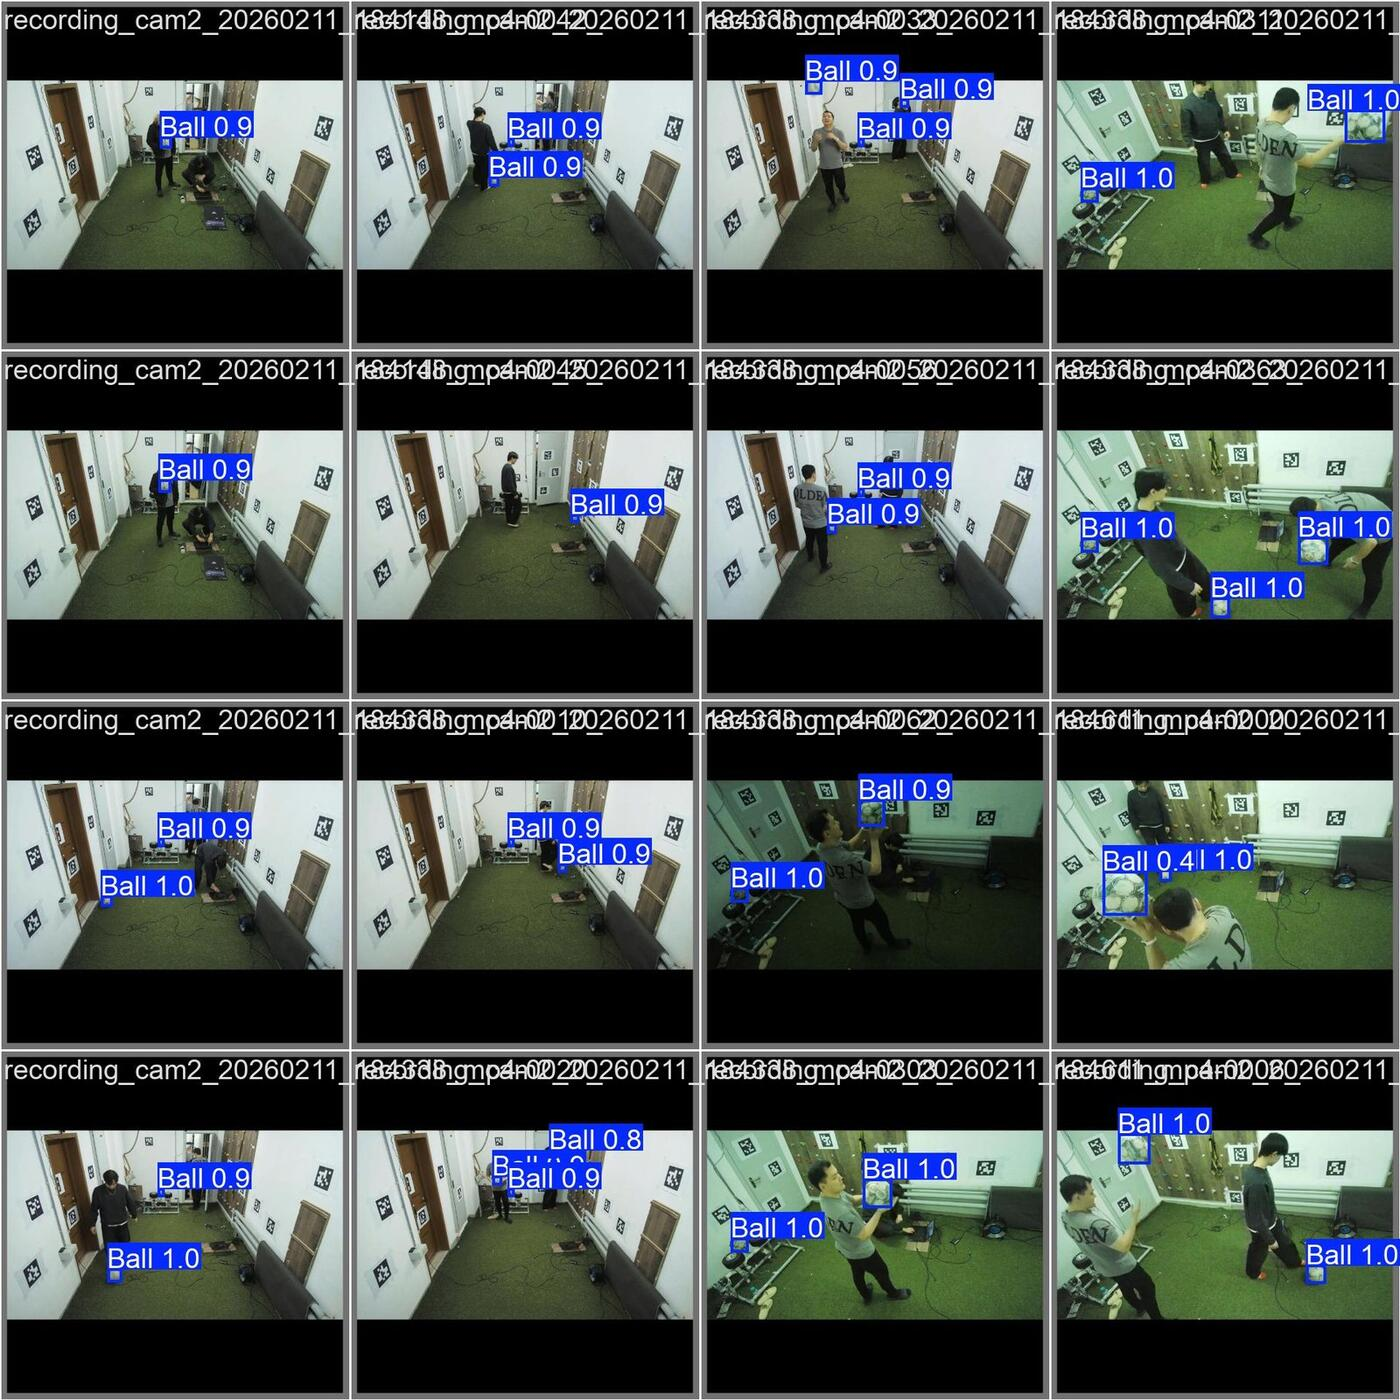
\includegraphics[width=0.9\textwidth]{figures/smoke_test_frame_1}
\caption{System architecture in action: live four-camera arena view showing YOLO ball detection (green bounding box), pose-skeleton overlay (COCO 17-keypoint), and 3D triangulated positions during continuous operation.}
\label{fig:3_3}
\end{figure}

\section{Intrinsic Calibration Pipeline}

\subsection{Board Specification and Detection}

A ChArUco board of 5~columns~$\times$~7~rows of 21.5~cm squares is used. Embedded ArUco markers in alternate squares supply identifiers for partial-board detection. The capture script streams from all four cameras simultaneously, detects ChArUco corners in each frame, and automatically saves a frame whenever more than 25 corners are detected and the detection is stable for three seconds. This hands-free protocol ensures sufficient pose diversity without operator-timing errors.

\subsection{Calibration Procedure}

Each camera is calibrated independently. For each camera, OpenCV \cite{ref27} is used to estimate the intrinsic matrix $K$ and distortion coefficients ($k_1, k_2, p_1, p_2, k_3$) by minimising the reprojection error across all collected frames. The target is approximately 30 valid frames per camera; frames with fewer than 25 detected corners are dropped before calibration. The intrinsic calibration is performed at 1280~$\times$~720, the resolution at which the system operates: calibrating at a different resolution would introduce a scaling error in $f_x$, $f_y$, $c_x$, $c_y$ that would propagate as a systematic triangulation bias.

\subsection{Output and Validation}

The calibration outputs are per-camera $K$ matrices and distortion vectors stored as JSON files in \path{garage_lab_combined/cal/intrinsics/}. Per-camera reprojection error is computed across the full calibration set as a quality indicator; values in the range 2--8~pixels are considered acceptable for this application.

\section{Extrinsic Calibration Pipeline}

\subsection{AprilTag Detection}

Twenty-four AprilTag markers (family \texttt{tag36h11}, IDs 0--23, 21.5~cm side) are affixed to the arena walls at pre-measured world-frame positions stored in the calibration configuration. The script \texttt{calibrate\_extrinsics\_apriltag\_robust.py} runs AprilTag detection on still frames captured from each camera and assembles a set of PnP correspondences: for each detected tag corner, a 3D world position and a 2D image position.

\subsection{Robust PnP Optimisation}

Camera pose ($R$, $T$) is estimated for each camera by RANSAC PnP (\texttt{cv2.solvePnPRansac} with the EPnP solver) followed by iterative refinement. An outlier-rejection step using the Median Absolute Deviation (MAD) of the reprojection residuals discards observations whose residual exceeds $2.5\sigma_{\text{MAD}}$, where $\sigma_{\text{MAD}} = 1.4826 \cdot \mathrm{median}(|r - \mathrm{median}(r)|)$. Tags whose median residual exceeds 45~pixels are rejected outright. PnP is then re-solved on the surviving inlier set with \texttt{SOLVEPNP\_ITERATIVE}. The procedure is iterated until the inlier set stabilises. The result is, per camera, a rotation matrix $R$ and a translation vector $T$ defining the camera's pose in the world frame.

\subsection{Overlay Validation}

Extrinsic quality is validated visually by reprojecting the known AprilTag corner positions back into each camera image using the estimated $(K, R, T)$ and overlaying the reprojected corners on the captured frame. When the reprojected corners align tightly with the detected corners across all cameras, the calibration is considered valid. This validation is performed after any physical camera movement and before any data-collection session.

\section{Multi-Camera Synchronisation}

The four Hikvision DS-E12 cameras have no hardware synchronisation signal. Software synchronisation is achieved through a flashlight sync-marker protocol: a hand-held flashlight is flashed briefly at the start of each recording session, creating a brightness spike that is detectable in all four streams. Frame alignment is performed by locating the spike frame in each stream and offsetting the subsequent frames accordingly.

For ground-truth evaluation sessions, which use static holds of 3--4~seconds, a synchronisation accuracy of $\pm$2 frames (approximately 130~ms at 15~FPS) is acceptable, as the target is stationary during the hold. For the dynamic validation clips, larger temporal offsets between cameras would induce parallax artefacts in the moving ball and would degrade triangulation accuracy.

The triangulation code requires a configurable minimum number of cameras (two for ball, three for joints). The number of cameras contributing to each frame is recorded for post-hoc analysis.

\section{3D Triangulation}

\subsection{Ball Triangulation}

For each frame in which the ball is detected in two or more cameras with confidence above the configured threshold (0.25--0.45 depending on the experiment), the bounding-box centres are passed through undistortion and combined into a homogeneous DLT system. Stacking the per-camera linear constraints into a matrix $A$, the 3D point $\mathbf{X}$ is the right-singular vector of $A$ corresponding to the smallest singular value \cite{ref1}.

\subsection{Robust Ball Triangulation}

A na\"{i}ve DLT solution is sensitive to a single mis-detected camera (e.g.\ a body or a cone mistaken for the ball). The live runtime therefore wraps the SVD solve in an iterative reprojection-error-rejection scheme (\texttt{robust\_triangulate\_ball}). On each iteration, the current 3D estimate is projected back into every contributing camera; the camera with the largest reprojection error is removed if that error exceeds the per-camera threshold (default 25~pixels). The SVD is re-solved, and the loop terminates when every remaining camera is within tolerance. A minimum of two cameras is enforced; if the iteration would drop below this minimum, the frame is rejected and the runtime falls back to a Kalman-filter coast (Section~3.9).

In addition, candidate selection \emph{before} triangulation applies three flag-guarded gates that operate on the raw YOLO bounding boxes per camera: a maximum bounding-box side gate (default 220~pixels), which rejects oversized blobs corresponding to bodies, cones, or markers misclassified as the ball; an optional minimum bounding-box side gate, which suppresses detector-noise micro-boxes; and a Kalman-distance gate that, when the ball Kalman filter is locked, prefers candidates within a configurable pixel radius of the predicted reprojection. Falling back to the highest-confidence box when no candidate is within the gate ensures that re-acquisition after long drops still works.

\subsection{Single-Camera Geometric Fallback}

When fewer than two cameras observe the ball, multi-view triangulation is geometrically impossible. For ball tracking only (and never for joints), a flag-guarded single-camera fallback is available: the undistorted ray from the one observing camera is intersected with a target Z plane derived either from the predicted Kalman filter Z-value or, for cold-start frames, from a configured floor plane. The fallback is capped at a maximum number of consecutive single-camera frames to prevent depth drift without geometric constraint, and is only enabled where bounce-heavy or low-visibility scenarios require it. The multi-view path is unchanged.

\subsection{Pose Joint Triangulation}

For each COCO keypoint, the same DLT/SVD procedure is followed using the per-camera 2D keypoint coordinate from each camera in which the joint confidence exceeds the pose-confidence threshold (0.35) and the joint is observed by at least three cameras. The minimum of three cameras for joints, compared with two for the ball, reflects the higher noise floor of learned keypoint estimates.

\subsection{Quality Filtering}

After triangulation, two filters are applied. \textbf{Reprojection-error check:} the triangulated 3D point is projected back into each contributing camera using the known $(K, R, T)$. If the pixel distance between the projected position and the original detection exceeds a per-experiment threshold (14--25~pixels), the point is rejected. \textbf{Adaptive EMA smoothing:} accepted 3D points are smoothed by an Exponential Moving Average with base coefficient $\alpha = 0.25$. When the per-frame jump $\|\mathbf{x}_t - \hat{\mathbf{x}}_{t-1}\|$ exceeds a configurable threshold (80~mm), $\alpha$ is boosted to 0.9 so that fast motion is not over-smoothed. The smoothed position is then handed to the Kalman filter.

\section{Ballistic Solver and Targeting Logic}

\subsection{Target Vector Computation}

The ballistic solver takes as input the corrected, predicted 3D world-frame target position $T = (T_x, T_y, T_z)$ in millimetres, sourced from the joint-specific Kalman filter (Section~3.9). The BLM pivot point is a fixed, calibrated world-frame coordinate $B = (B_x, B_y, B_z) = (600, 1560, 500)$~mm.

The targeting vector from launcher to target is:

\begin{equation}
\Delta X = T_x - B_x \label{eq:3_1}
\end{equation}
\begin{equation}
\Delta Y = T_y - B_y \label{eq:3_2}
\end{equation}
\begin{equation}
\Delta Z = T_z - B_z \label{eq:3_3}
\end{equation}

The horizontal ground distance is:

\begin{equation}
D_{\text{horiz}} = \sqrt{\Delta X^2 + \Delta Y^2} \label{eq:3_4}
\end{equation}

\subsection{Yaw Angle Computation}

The required yaw (horizontal rotation) angle of the launcher to point at the target in the arena plane is:

\begin{equation}
\theta_{\text{yaw}} = \mathrm{atan2}(\Delta Y, \Delta X) \label{eq:3_5}
\end{equation}

This is measured relative to the launcher's reference direction (positive X). The result is converted to degrees and offset by the configured \texttt{\detokenize{--yaw-trim-deg}} parameter, which compensates for any mechanical zero offset produced by the stepper-motor homing procedure.

\subsection{Pitch Angle Computation}

The pitch angle is derived from the projectile-motion equations~(\ref{eq:2_2})--(\ref{eq:2_4}). For a target at horizontal distance $D_{\text{horiz}}$ and height difference $\Delta Z$, the required pitch angle $\theta_{\text{pitch}}$ at a given initial ball speed $v_0$ satisfies:

\begin{equation}
\Delta Z = D_{\text{horiz}} \cdot \tan(\theta_{\text{pitch}}) - \frac{g \cdot D_{\text{horiz}}^2}{2 \cdot v_0^2 \cdot \cos^2(\theta_{\text{pitch}})} \label{eq:3_6}
\end{equation}

This is a transcendental equation in $\theta_{\text{pitch}}$. For arena distances of 2000--5000~mm and the chosen ball speeds, the discriminant of the equivalent quadratic in $\tan(\theta)$ is non-negative for in-range targets and yields two valid solutions: a low arc and a high arc. The low-arc solution is preferred because it minimises flight time and therefore the targeting uncertainty introduced by athlete movement during flight. The result is offset by the \texttt{\detokenize{--pitch-trim-deg}} parameter to remove mechanical zero offset.

\subsection{Wheel RPM Computation}

The wheel RPM is proportional to the desired initial ball speed $v_0$. The empirical RPM-to-velocity mapping is established from controlled calibration shots; a runtime parameter (\texttt{\detokenize{--speed-scale}}) supports adjustment without firmware changes. The full empirical RPM-to-velocity calibration over the 500--1200~RPM range is identified as future work in Section~6.4.

\subsection{Why Real-Time Targeting Is Non-Trivial}

The targeting computation is not a look-up table; it is a real-time constrained optimisation. First, the target $T$ updates every frame at 15~FPS, so the solver must complete within a single frame time (approximately 67~ms) to avoid issuing stale commands. Second, gravity couples pitch and ball speed: the same target can be reached at multiple $(\theta, v_0)$ combinations, and the solver must select the physically valid low-arc solution and verify that it lies within the mechanical range of the gimbal ($\pm 30^\circ$). Third, the stepper has finite step resolution, so the solver rounds to the nearest achievable step and logs the angular residual error for post-session analysis. Fourth, the BLM's mechanical zero (the position after \texttt{setzero}) must be registered to the world coordinate system; this registration is performed through the yaw and pitch trim calibration, which is itself validated in the aim-only tests of Chapter~5.

\subsection{Dynamic Target Tracking Behaviour}

The system operates as a state machine with three targeting states. In the \textbf{ACQUIRING} state, the joint is detected by fewer than the minimum required cameras or its EMA-filtered position has not yet stabilised; no command is dispatched. In the \textbf{LOW\_CONFIDENCE} state, the detection confidence is below threshold or the joint position has changed by more than 50~mm in the most recent ten frames; the last valid command is held and the decision is logged as \texttt{LOW\_CONFIDENCE}. In the \textbf{READY} state, the joint position is stable (movement below 50~mm over ten frames) and confidence is above threshold; the ballistic solve is executed and the serial command is dispatched. A transition from READY back to ACQUIRING occurs when the joint disappears from the camera views (for example, the athlete moves behind a wall or crouches below the field of view). Firing is permitted only in the READY state with the E-STOP cleared.

\section{Predictive Tracking with a Kalman Filter}

The smoothed 3D position from Section~3.7 is fed into a per-joint and per-ball Kalman filter implemented as the \texttt{JointKalmanFilter} class. The motion model is constant velocity (CV) with state $\mathbf{x} = [X, Y, Z, \dot{X}, \dot{Y}, \dot{Z}]^\top \in \mathbb{R}^{6}$, transition matrix
\[
F(\Delta t) =
\begin{bmatrix}
I_3 & \Delta t \cdot I_3 \\
0_3 & I_3
\end{bmatrix},
\]
and process noise driven by a piecewise-constant white-noise acceleration model with intensity $q$ (process-noise parameter).

The measurement model observes only the position component, $H = \begin{bmatrix} I_3 & 0_3 \end{bmatrix}$, with measurement-noise covariance $R_{\text{KF}} = r \cdot I_3$. The standard predict and update steps,
\begin{align*}
\mathbf{x}^{-} &= F \mathbf{x},\quad P^{-} = F P F^\top + Q,\\
K &= P^{-} H^\top (H P^{-} H^\top + R_{\text{KF}})^{-1},\\
\mathbf{x} &= \mathbf{x}^{-} + K (\mathbf{z} - H \mathbf{x}^{-}),\quad P = (I - K H) P^{-},
\end{align*}
are executed at every frame in which a measurement is available. A \textbf{predict-ahead} step uses $F(\Delta t_{\text{pred}})$ without an update to extrapolate the state into the future; the predicted position is shipped alongside the current position in the UDP target packet, allowing the launcher runtime to compensate for the projectile flight time.

The CV process- and measurement-noise parameters are tuned per task. For joint tracking, the tuned values are $q = 500$~mm$^{2}$/s$^{4}$ and $r = 10$~mm$^{2}$ at a predict-ahead horizon of 400~ms (Section~5.7). For the ball, a more reactive $q = 800$, $r = 25$ pair is used, complemented by a maximum-physical-speed gate (40~m/s) and a coast-through-drop window of six frames during which the filter continues to predict in the absence of measurements.

When a frame contains no triangulated measurement (for example, all cameras lost the joint), the Kalman filter executes a predict step only, with optional velocity damping during the coast. After a configurable number of consecutive coast frames, the filter is reset to the next valid measurement to avoid blending stale velocity into a re-acquisition.

\section{BLM Firmware: \texttt{control\_12\_full.ino}}

The firmware is a cooperative state machine running on ESP32 core~1, with stepper step-pulse generation in a hardware-timer interrupt service routine and UART command parsing in the main \texttt{loop()}. There is no operating system; the real-time guarantees required (pulse jitter $<$~50~$\mu$s) are easier to meet in a bare-loop design with explicit critical sections.

\subsection{Finite State Machine}

The firmware FSM has three primary states whose transitions are guarded by sensor events (limit-switch readings) or timers (the 10~s dispense fallback), as illustrated in the following transition diagram:

\begin{center}
\small
\setlength{\tabcolsep}{5pt}
\newcommand{\fsmstate}[1]{\fbox{\strut\texttt{#1}}}
\begin{tabular}{ccccc}
\fsmstate{IDLE} & $\xrightarrow{\text{\ttfamily reload}}$ &
\fsmstate{RETRACTING} & $\xrightarrow{\text{\ttfamily back\_LOW}}$ &
\fsmstate{DISPENSING} \\
&&&& $\downarrow\ \text{\ttfamily ball\_LOW or 10 s}$ \\
&&&& \fsmstate{IDLE}
\end{tabular}

\vspace{0.5em}

\begin{tabular}{ccccc}
\fsmstate{IDLE} & $\xrightarrow{\text{\ttfamily shoot (RPM >= 400)}}$ &
\fsmstate{SHOOTING} & $\xrightarrow{\text{\ttfamily pusher\_fwd; front\_LOW}}$ &
\fsmstate{IDLE}
\end{tabular}
\end{center}

Each transition is gated by a sensor event or a timeout; commands set the desired state, but the actual state is confirmed by sensors. This discipline allows the system to recover from a jammed ball: the FSM stays in DISPENSING until the ball-limit switch confirms a ball is in position, and if the timer expires the FSM returns to IDLE rather than hanging.

\subsection{Firmware-Level Interlocks}

Three safety interlocks are enforced inside the firmware itself. The \textbf{RPM gate}: \texttt{shoot} is rejected if either flywheel reads below 400~RPM. This is a second line of defence behind the supervisor's RPM check, ensuring that a stale or malicious \texttt{shoot} command from a raw terminal cannot fire with cold flywheels. The \textbf{angle clamp}: while the supervisor is the authoritative clamp, the firmware additionally clips \texttt{set} commands to $\pm 30^\circ$ to survive supervisor bugs. The \textbf{pusher enable} discipline: \texttt{nENABLE} is held LOW (driver active) only in the three non-IDLE states; in IDLE, the driver is disabled so the coil is cold.

\subsection{Telemetry}

The firmware streams \texttt{L:}$\langle$rpm$\rangle$ \texttt{R:}$\langle$rpm$\rangle$ telemetry lines over the UART, but only while the FSM is in IDLE. During pusher motion, the current draw briefly couples into the logic ground and corrupts the UART; telemetry is therefore state-gated and resumes the moment motion ends. The supervisor's RPM-gate check parses the most recent telemetry line and uses it as the live RPM for the gate condition.

\section{Communication Stack}

\subsection{Physical and Link Layers}

The supervisor-to-microcontroller link is a USB 2.0 Full-Speed UART through a CP2102 or CH340 bridge on the ESP32 development board. The link operates at \textbf{921~600~baud} with no flow control. Framing is newline-terminated ASCII. The 921~600~baud choice means that a typical command-plus-telemetry exchange fits inside a 1~ms window, which is small relative to the 67~ms perception cycle. At the precursor laboratory's 115~200~baud, the \texttt{info} response (approximately 200~bytes) consumed approximately 17~ms, a non-negligible fraction of the perception cycle; at 921~600~baud the same response consumes approximately 2~ms. ASCII framing is preferred over binary because the command set is small enough that compaction saves nothing meaningful at this rate, and human-readable serial output is a substantial debuggability win during bring-up.

\subsection{Why USB-Serial Is the Primary Link}

The precursor bachelor project used Bluetooth Low Energy (BLE, Nordic UART Service) as the primary command channel. This thesis migrates back to USB-serial as primary because: (i) USB UART delivers consistent sub-millisecond receive latency, while BLE connection intervals are negotiated and a slow peer can extend them to 30~ms; (ii) BLE Maximum Transmission Unit (MTU, $\sim$244~bytes after ATT overhead) and the 7.5~ms minimum connection interval place a ceiling on telemetry bandwidth that is awkward for the \texttt{info} string; (iii) USB has a single failure mode (one cable; no pairing state machine, no bond-storage corruption); (iv) \texttt{pyserial} is a smaller dependency than \texttt{bleak}. BLE remains compiled-in on the ESP32 as a backup channel (advertising name \texttt{RoboLauncher}) for a future mobile-app use case, which is not in the scope of this thesis.

\subsection{UDP Channels}

Two UDP channels carry runtime data. Port \textbf{5005} carries the launcher target stream from the live viewer to the launcher runtime: a JSON packet per frame containing the ball position, the per-joint current and predicted positions, and per-joint confidence and camera-count metadata. Port \textbf{5006} carries the voice-bridge stream from the offline ASR producer (Section~3.12) to the runtime, delivering recognised utterances as short tokens. Both channels are intra-host (loopback by default) but can be routed across a trusted local network when the hosts are physically separated.

\subsection{Decision Log}

Every decision the supervisor makes about whether to issue an actuation command is recorded to a JSON Lines (JSONL) file with the fields \path{timestamp}, \path{input_joint_name}, \path{raw_world_xyz_mm}, \path{transformed_launcher_xyz}, \path{calculated_pitch_yaw_v}, \path{decision} (one of \path{OK}\,/\,\path{OUT_OF_RANGE}\,/\,\path{LOW_CONFIDENCE}\,/\,\path{ESTOP}), and \path{execution_time_ms}. This log provides full traceability of every aim or fire decision and is used both for post-session analysis and for the integration-test evidence of Appendix~A.

\section{Multi-Modal Voice-Command Integration}

The runtime exposes a multi-modal control front-end that complements the keyboard input with offline speech recognition. An offline Vosk \cite{ref41_vosk} acoustic model recognises a 16-phrase grammar that maps natural utterances to COCO joint names (e.g.\ \textit{``right knee''}, \textit{``left shoulder''}, \textit{``nose''}) and to control verbs (\texttt{shoot}, \texttt{reload}, \texttt{pause}, \texttt{resume}, \texttt{quit}).

The ASR producer runs in a separate Python interpreter, not in the main runtime's environment. The recognised tokens are forwarded over UDP port~5006 to the live runtime, which feeds them into the same target-selection and command-dispatch path used for keyboard input. This isolation is deliberate: the audio I/O subsystem (\texttt{pyaudio}, \texttt{vosk}, audio device drivers) has a substantial dependency footprint and a different failure grammar from the perception stack, and isolating it through UDP avoids contaminating the production runtime's environment.

A complementary auto-reload mode is available in the follow-mode runtime: after a successful \texttt{shoot}, the system automatically issues \texttt{reload}, keeps the wheels spinning, and retains the current joint target so that the next \texttt{go} (or voice equivalent) fires the same joint. This enables a hands-free rapid-fire training cadence without keyboard interaction. The voice front-end and auto-reload mode operate behind the same safety gates as keyboard control; they do not bypass the RPM gate, the zone gate, or the E-STOP latch. Closed-loop voice-controlled firing on a moving subject is identified as future work in Section~6.4.

\section{Ball Detection Robustness}

The ball detector is an Ultralytics YOLO model trained on a domain-specific dataset and deployed via a TensorRT FP16 dynamic-batch engine \cite{ref38_tensorrt}. The training and validation curves for the ball detector are reported in Appendix~E.

Three flag-guarded gates are applied to the per-camera detector output before triangulation, in the order listed:

\begin{enumerate}
    \item \textbf{Maximum bounding-box side gate} (\texttt{\detokenize{--ball-max-box-side-px}}, default 220). A tennis-sized training ball at the operating distances has a bounding-box side below approximately 120~pixels; the 220-pixel cap rejects body-sized blobs and large markers misclassified as the ball, while leaving close-range legitimate detections untouched.
    \item \textbf{Minimum bounding-box side gate} (\texttt{\detokenize{--ball-min-box-side-px}}, default off). When enabled, this rejects detector-noise micro-boxes (typically far-distance speckle) whose side is below the configured threshold.
    \item \textbf{Kalman-distance gate} (\texttt{\detokenize{--ball-kf-gate-px}}, default 150). When the ball Kalman filter is locked, per-camera selection prefers the candidate whose centre lies within the configured pixel radius of the predicted reprojection. If no candidate is within the gate, the gate falls back to the highest-confidence box, ensuring that re-acquisitions after long drops still work.
\end{enumerate}

The detector's input resolution can also be configured: a default of 672 is used, but a larger 960 input recovers approximately 40 percentage points of detection rate on the camera that observes a low bounce, at a cost of approximately 8~ms additional inference latency per four-camera batch. The trade-off is documented in Section~5.8.

\section{Safety Architecture}

The safety design follows a defence-in-depth pattern: every command that would cause unsafe motion must defeat all of the gates listed below.

\subsection{Layered Interlocks}

\begin{itemize}
    \item \textbf{L1 Zone gate.} The triangulated target must lie within a per-joint safe zone derived from the ground-truth survey. Out-of-zone targets are rejected with \texttt{OUT\_OF\_RANGE}.
    \item \textbf{L2 Confidence gate.} The target must be observed by at least three cameras and the per-joint confidence must exceed 0.45. Otherwise the decision is \texttt{LOW\_CONFIDENCE} and the last valid command is held.
    \item \textbf{L3 Stability gate.} The sliding-window standard deviation of the target position must be below a configurable threshold; jittery targets are rejected.
    \item \textbf{L4 Angle clamp.} Pitch is clamped to $[0^\circ, 30^\circ]$ and yaw to $[-30^\circ, 30^\circ]$ in the supervisor before transmission, and again in the firmware as a second line of defence.
    \item \textbf{L5 RPM gate.} \texttt{shoot} is permitted only when both flywheel telemetry readings are at or above 400~RPM; this is enforced in both the supervisor and the firmware.
    \item \textbf{L6 Arm state.} In follow mode, the operator must explicitly type \texttt{reload} (or speak the voice equivalent) before the first aim is dispatched; aim is suppressed until armed.
    \item \textbf{L7 Confirmation.} In the live aim test (single-shot mode), the operator must type the full word \texttt{yes} to confirm fire after a successful aim.
    \item \textbf{L8 Hardware E-STOP.} The normally-closed mushroom switch latches the 24~V motor rail off in $<$~100~ms.
    \item \textbf{L9 Link-loss safe stop.} On UDP timeout or serial disconnection, the supervisor automatically sends \texttt{stop} and \texttt{set 0 0 0 0}.
    \item \textbf{L10 Exception path.} Any uncaught Python exception in the supervisor triggers the same safe-stop sequence.
\end{itemize}

\subsection{Standards Alignment}

The safety design is informed by, and consistent with, the following standards: ISO~12100 \cite{ref22} (general machinery safety principles, applied to the L1--L10 hazard analysis), ISO~13849-1 \cite{ref44_iso13849} (the E-STOP at L8 implements a Category~1 stop by removing energy from the motor rail), IEC~60204-1 \cite{ref45_iec60204} (control-circuit wiring, 24~V/50~A fuse sizing, ground-loop topology), and ISO~10218-1 \cite{ref26} (exclusion-zone discipline during controlled fire, with the operator behind the launcher and no person down-range unless the operator is the designated target).

\subsection{Six-Stage Integration Checklist}

Integration of the full system follows a mandatory staged protocol to prevent unsafe operation before each component has been validated in isolation. The stages are: \textbf{S0 Preflight} (camera stream, calibration files, serial line); \textbf{S1 ESP32-only} (motor commands via direct serial terminal, no camera or BLM active); \textbf{S2 Runtime without cameras} (synthetic UDP target packets to verify solver and gate logic); \textbf{S3 Live aim-only} (full pipeline active, motors commanded to correct angles, no ball loaded); \textbf{S4 Safety verification} (E-STOP, latch, link-loss, zone-rejection tests under live conditions); \textbf{S5 Controlled fire} (single shots with ball loaded, one at a time, operator present); \textbf{S6 Full-cycle reliability} (10 consecutive cycles without crash or unsafe behaviour). Each stage has defined pass criteria and an evidence requirement (terminal log, video, or JSONL record). A stage is not passed until all of its criteria are met. The full checklist is in Appendix~A; Stages~S0--S4 were completed on real hardware on 2026-04-09, and the integrated live test is reported in Section~5.9.
